\documentclass[12pt]{amsart}
\usepackage{tikz}
\usetikzlibrary {shapes.geometric}
\title{Activity 1.1}
\date{\today}
\begin{document}
% \maketitle
\part*{Triangular Numbers}
\begin{enumerate}
\item Write down the sequence that are formed by pentagons. Find the pattern in this sequence and see if the same can be done for other geometric objects.
\begin{figure}
    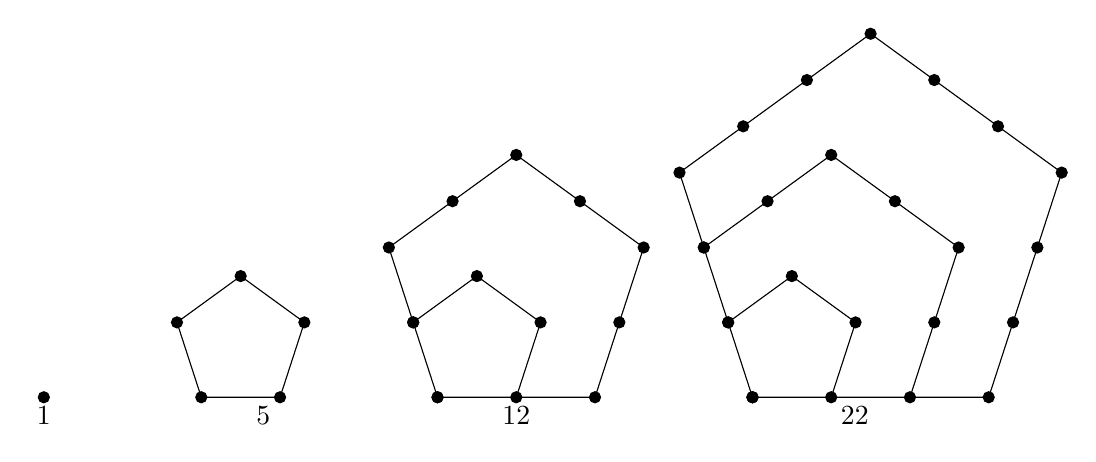
\begin{tikzpicture}
        \filldraw (0,0) node[below]{$1$} circle [radius=2pt];
        \filldraw (2,0) circle [radius=2pt] --++ (0:1)node[below left]{$5$} circle [radius=2pt] --++ (72:1) circle [radius=2pt] --++ (144:1) circle [radius=2pt] --++ (216:1) circle [radius=2pt] --++ (288:1) circle [radius=2pt];
        \filldraw (5,0) circle [radius=2pt] --++ (0:1) circle [radius=2pt] --++ (72:1) circle [radius=2pt] --++ (144:1) circle [radius=2pt] --++ (216:1) circle [radius=2pt] --++ (288:1) circle [radius=2pt];
        \filldraw (5,0) circle [radius=2pt] ++ (0:1)node[below]{$12$} --++ (0:1) circle [radius=2pt] --++ (72:1) circle [radius=2pt] --++ (72:1) circle [radius=2pt] --++ (144:1) circle [radius=2pt] --++ (144:1) circle [radius=2pt] --++ (216:1) circle [radius=2pt] --++ (216:1) circle [radius=2pt] --++ (288:1) circle [radius=2pt];
        \filldraw (9,0) circle [radius=2pt] --++ (0:1) circle [radius=2pt] --++ (72:1) circle [radius=2pt] --++ (144:1) circle [radius=2pt] --++ (216:1) circle [radius=2pt] --++ (288:1) circle [radius=2pt];
        \filldraw (9,0) circle [radius=2pt] ++ (0:1)node[below right]{$22$} --++ (0:1) circle [radius=2pt] --++ (72:1) circle [radius=2pt] --++ (72:1) circle [radius=2pt] --++ (144:1) circle [radius=2pt] --++ (144:1) circle [radius=2pt] --++ (216:1) circle [radius=2pt] --++ (216:1) circle [radius=2pt] --++ (288:1) circle [radius=2pt];
        \filldraw (9,0) circle [radius=2pt] ++ (0:2) --++ (0:1) circle [radius=2pt] --++ (72:1) circle [radius=2pt] --++ (72:1) circle [radius=2pt] --++ (72:1) circle [radius=2pt] --++ (144:1) circle [radius=2pt] --++ (144:1) circle [radius=2pt] --++ (144:1) circle [radius=2pt] --++ (216:1) circle [radius=2pt] --++ (216:1) circle [radius=2pt] --++ (216:1) circle [radius=2pt] --++ (288:1) circle [radius=2pt];
      \end{tikzpicture} 
\end{figure}
\end{enumerate}
\end{document}
